% =============================================================================
% INF-221 Algoritmos y Complejidad -- Tarea 1 -- Semestre 2026-2
% Autor: Kurt Wiederhold   Rol: 202473528-4
% Seccion: Resultados y Analisis (extension maxima: 4 paginas)
%
% NOTA: todas las figuras, todas las tablas y todos los numeros citados en el
% texto de esta seccion (macros \Sort... y \Mat...) se generan automaticamente
% con los scripts scripts/plot_generator.py de cada experimento a partir de
% los CSV de mediciones. No hay ningun numero escrito a mano.
% =============================================================================

Figuras y tablas se generan desde los CSV con \texttt{plot\_generator.py} y
quedan en \texttt{data/plots/} de \texttt{code/sorting} y de
\texttt{code/matrix\_multiplication}.

\subsection{Ordenamiento de arreglos}

\begin{figure}[H]
  \centering
  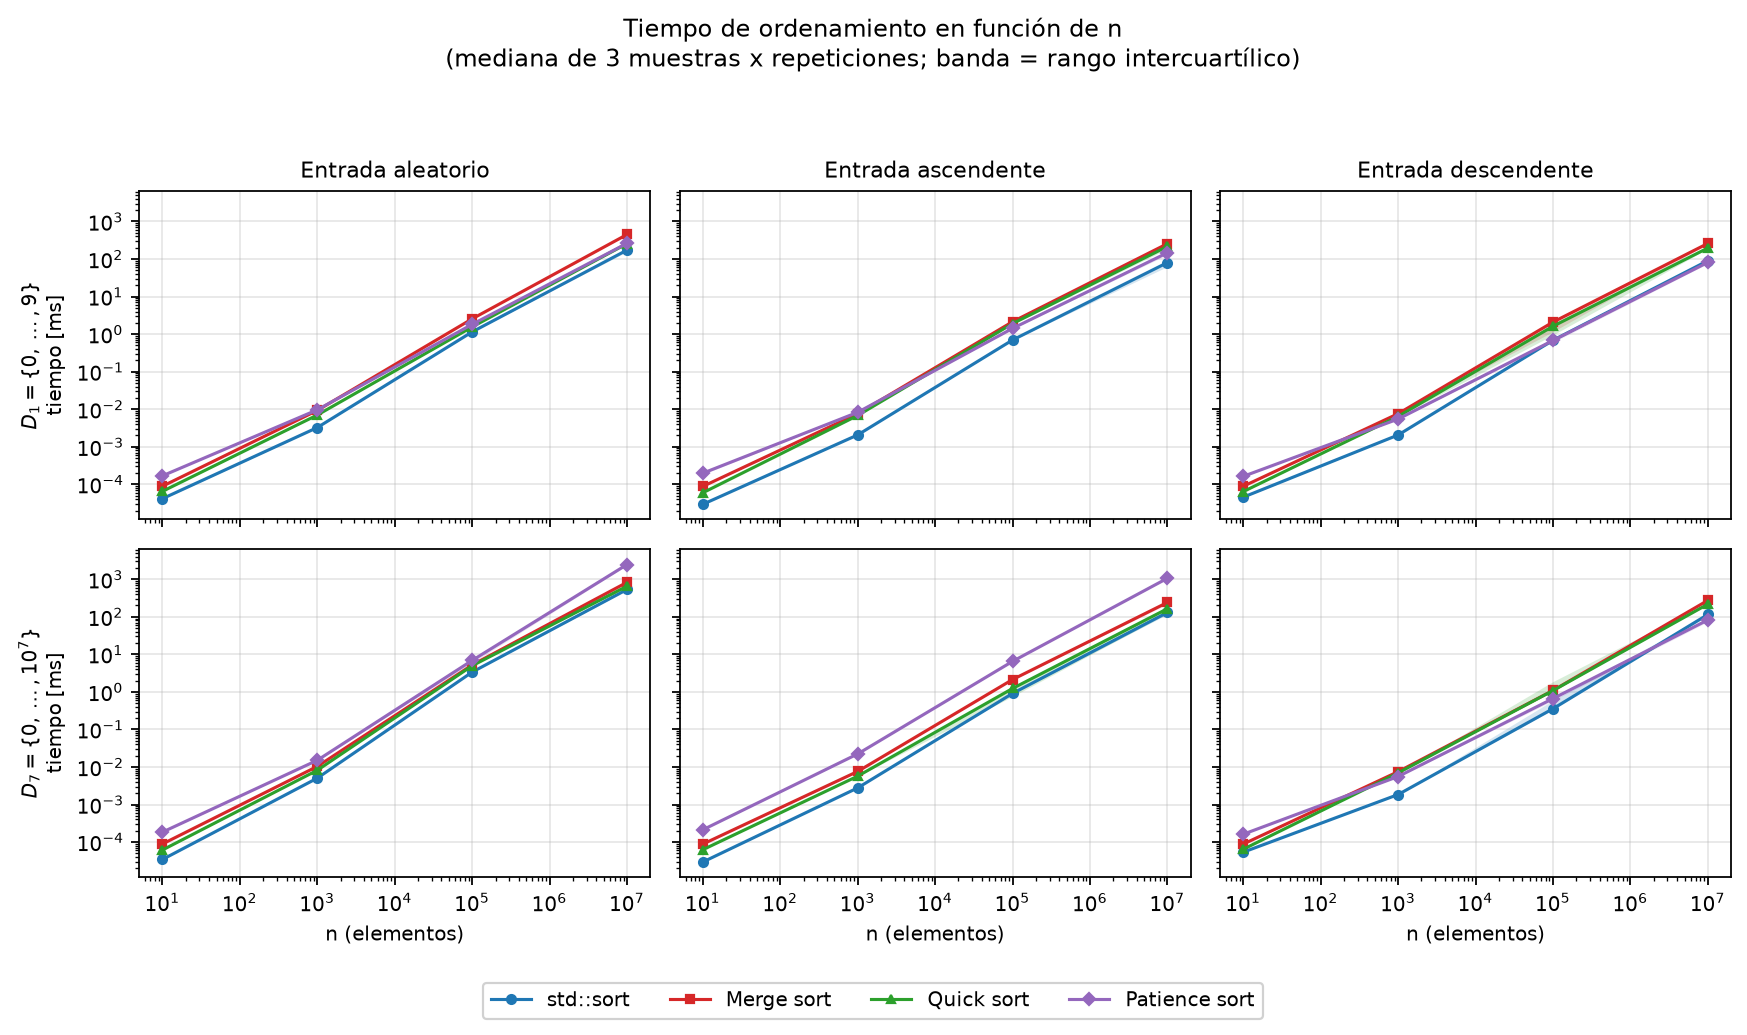
\includegraphics[width=0.48\textwidth]{../code/sorting/data/plots/sorting_time_vs_n.png}
  \caption{Tiempo frente a $n$ (doble logarítmica), por orden inicial
  (columnas) y dominio (filas). Las curvas son casi paralelas: lo que separa a
  los algoritmos es el factor constante, no el orden de crecimiento.}
  \label{fig:sorting-time}
\end{figure}

% =============================================================================
% INF-221 Algoritmos y Complejidad -- Tarea 1 -- Semestre 2026-2
% Autor: Kurt Wiederhold   Rol: 202473528-4
%
% ARCHIVO GENERADO AUTOMATICAMENTE por code/sorting/scripts/plot_generator.py
% a partir de data/measurements/sorting_measurements.csv. No editar a mano:
% se regenera con `make plots`.
% =============================================================================
\begin{table}[H]
\centering
\small
\caption{Tiempo mediano [ms], entrada \emph{aleatoria} con dominio $D_7$ (mediana sobre las tres muestras y todas las repeticiones).}
\label{tab:sorting-time}
\begin{tabular}{lrrrr}
\hline\hline
Algoritmo & $n=10^{1}$ & $n=10^{3}$ & $n=10^{5}$ & $n=10^{7}$ \\
\hline
std::sort & $3{,}44\times 10^{-5}$ & $5{,}05\times 10^{-3}$ & 3{,}37 & 535 \\
Merge sort & $8{,}90\times 10^{-5}$ & 0{,}0104 & 5{,}21 & 829 \\
Quick sort & $6{,}16\times 10^{-5}$ & $8{,}19\times 10^{-3}$ & 4{,}98 & 653 \\
Patience sort & $1{,}84\times 10^{-4}$ & 0{,}0151 & 6{,}90 & 2469 \\
\hline\hline
\end{tabular}
\end{table}


En escala doble logarítmica una ley de potencias es una recta, y en la
\Cref{fig:sorting-time} las cuatro curvas son rectas casi paralelas: ningún
algoritmo cambia de orden. El ajuste $t=c\,n^{p}$ de la
\Cref{tab:sorting-exponents} lo confirma, con exponentes entre $\SortExpMin$ y
$\SortExpMax$ en torno al $\SortExpNlogn$ de $n\log_2 n$ en este rango. La
notación asintótica acierta, y es todo lo que acierta: no distingue entre las
cuatro curvas, y esas diferencias son grandes.

\textbf{Las constantes ocultas.} En la \Cref{tab:sorting-time}, para
$n=10^{7}$ con entrada aleatoria, quick sort tarda $\SortRatioQuickStd$ veces
lo que \texttt{std::sort}, merge sort $\SortRatioMergeStd$ y patience sort
$\SortRatioPatienceStd$. Los cuatro son $\Theta(n\log n)$ y aun así el peor
cuesta $\SortWorstOverBest\times$ el mejor. La ventaja de \texttt{std::sort}
es de ingeniería, no de orden: introsort remata los subarreglos de tamaño
$\le16$ con una única pasada de inserción sobre todo el
arreglo~\cite{musser1997,cppreference_sort}.

\begin{figure}[H]
  \centering
  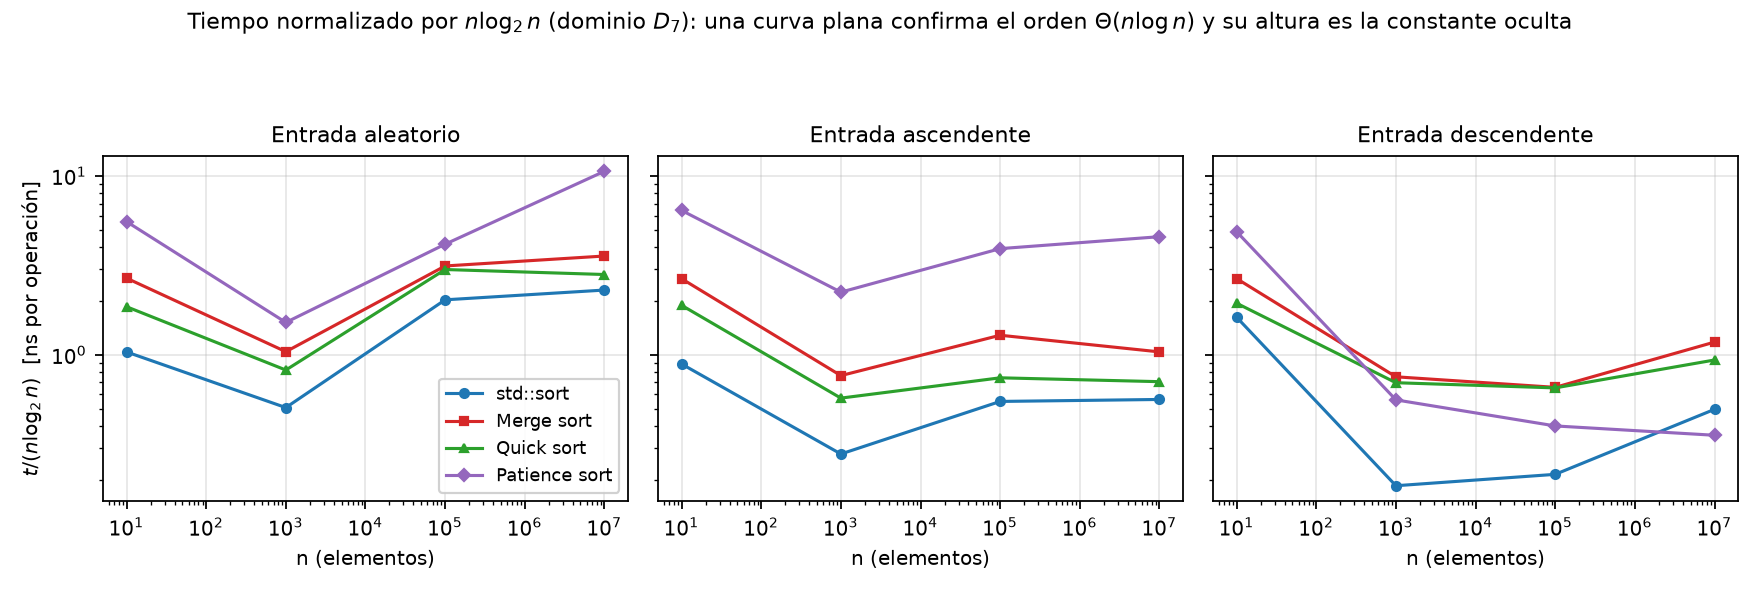
\includegraphics[width=0.50\textwidth]{../code/sorting/data/plots/sorting_normalized_nlogn.png}
  \caption{Tiempo dividido por $n\log_2 n$ (ns por operación). Con costo
  uniforme por operación la curva sería horizontal, a la altura de la
  constante oculta.}
  \label{fig:sorting-normalized}
\end{figure}

\textbf{El costo por operación no es constante.} Las curvas de la
\Cref{fig:sorting-normalized} no son horizontales: entre $n=10^{3}$ y
$n=10^{5}$ el costo por operación de \texttt{std::sort} sobre entrada aleatoria
salta de $\SortStdNsSmall$ a $\SortStdNsMid$~ns, un factor $\SortStdNsFactor$.
La interpretación más plausible es la jerarquía de memoria: $10^{3}$ enteros
ocupan 4~KiB y caben en L1 (32~KiB); $10^{5}$ ocupan 400~KiB y sólo caben en
L2 (1~MiB); $10^{7}$ ocupan 40~MiB y ya no caben en L3 (32~MiB), y un fallo de
L3 cuesta unas dos órdenes de magnitud más que un acierto de
L1~\cite{drepper2007} (interpretación: aquí no se miden fallos de caché). A
partir de $n=10^{5}$ la curva se aplana y ahí sí se lee la constante de cada
algoritmo.

\textbf{La forma de la entrada importa, incluso donde la teoría dice que no.}
Con $n=10^{7}$ y dominio $D_7$, pasar de la entrada aleatoria a la más favorable
de las dos ordenadas divide el tiempo por $\SortOrderGainStd$ en
\texttt{std::sort}, $\SortOrderGainQuick$ en quick sort y $\SortOrderGainMerge$
en merge sort. Este último es el caso interesante: es deliberadamente
insensible a los datos (sin el atajo que salta la mezcla de mitades ya
ordenadas) y mueve los mismos elementos con cualquier permutación. Dos efectos
que la cuenta de operaciones no ve pueden explicarlo: con entrada ordenada cada mezcla agota primero el tramo izquierdo
(exactamente la mitad de las comparaciones) y \texttt{a[i] <= a[j]} es siempre
verdadera, lo que favorecería al predictor de saltos (hipótesis no medida). El dominio produce un efecto análogo: con $n$ fijo y entrada
aleatoria, pasar de $D_1$ a $D_7$ multiplica el tiempo por
$\SortDomainFactorStd$ en \texttt{std::sort} y por $\SortDomainFactorPatience$
en patience sort, con el mismo $n$.

\textbf{Patience sort: el peor caso medido no es el peor caso teórico.} Con
entrada descendente todo cae en una sola pila, la mezcla es trivial y el
algoritmo es $\Theta(n)$: tarda $\SortPatDescMs$~ms y gana a los
$\SortStdDescMs$~ms de \texttt{std::sort}. La teoría señala como peor caso la
entrada ascendente, que abre una pila por valor distinto
($k\approx\SortPatPilesTheory$ millones en $D_7$; los repetidos comparten
pila) y sube a $\SortPatAscMs$~ms. Pero el peor caso \emph{medido} es la
entrada aleatoria: $\SortPatRandMs$~ms, $\SortPatRandOverAsc$ veces la
ascendente, pese a generar sólo $k\approx2\sqrt{n}\approx\SortPatPilesRandom$
pilas. La hipótesis más plausible es de nuevo la memoria: con pocas pilas
largas, la mezcla sigue el puntero \texttt{below[i]} hacia una posición
\emph{aleatoria} de dos arreglos de 40~MiB (dos accesos sin localidad por
elemento), mientras que con la entrada ascendente las pilas tienen uno o dos
elementos y la búsqueda binaria recorre siempre el mismo camino. La razón
entre su mejor y su peor caso medidos es $\SortPatWorstBest$, frente a
$\SortOthersWorstBestMin$--$\SortOthersWorstBestMax$ de los otros tres.

% =============================================================================
% INF-221 Algoritmos y Complejidad -- Tarea 1 -- Semestre 2026-2
% Autor: Kurt Wiederhold   Rol: 202473528-4
%
% ARCHIVO GENERADO AUTOMATICAMENTE por code/sorting/scripts/plot_generator.py
% a partir de data/measurements/sorting_measurements.csv. No editar a mano:
% se regenera con `make plots`.
% =============================================================================
\begin{table}[H]
\centering
\small
\caption{Exponente empírico $p$ de $t = c\,n^{p}$ (mínimos cuadrados en log-log, dominio $D_7$). Un $\Theta(n\log n)$ debe dar $p\approx1{,}14$, la pendiente de $n\log_2 n$ en el rango medido. Entre paréntesis, $R^2$.}
\label{tab:sorting-exponents}
\begin{tabular}{lrrr}
\hline\hline
Algoritmo & aleatorio & ascendente & descendente \\
\hline
std::sort & 1{,}220 (0{,}997) & 1{,}123 (0{,}998) & 1{,}064 (0{,}989) \\
Merge sort & 1{,}180 (0{,}998) & 1{,}088 (0{,}998) & 1{,}082 (0{,}998) \\
Quick sort & 1{,}193 (0{,}997) & 1{,}079 (0{,}999) & 1{,}089 (0{,}999) \\
Patience sort & 1{,}202 (0{,}995) & 1{,}128 (0{,}999) & 0{,}960 (0{,}995) \\
\hline\hline
\end{tabular}
\end{table}


\textbf{Memoria.} La firma del \texttt{sort.cpp} entregado devuelve una copia
del arreglo, así que toda llamada asigna al menos $4n$ bytes; con ese piso, la
\Cref{tab:sorting-memory} separa los dos grupos que predice la teoría.
\texttt{std::sort} y quick sort dan exactamente $4n$: sólo la copia, sin memoria
auxiliar propia ($\Theta(1)$ más $\Theta(\log n)$ de pila, que este instrumento
no ve). Merge sort da $8n$: la copia más su búfer. Patience sort llega a $8n$
en el caso típico y a \SortPatMemWorst{} ($\SortPatMemWorstOverArray$ veces el
arreglo) en el ascendente $D_7$, por los $\approx\SortPatPilesTheory$ millones
de entradas del heap de mezcla: paga con memoria su ventaja en el caso
descendente.

% =============================================================================
% INF-221 Algoritmos y Complejidad -- Tarea 1 -- Semestre 2026-2
% Autor: Kurt Wiederhold   Rol: 202473528-4
%
% ARCHIVO GENERADO AUTOMATICAMENTE por code/sorting/scripts/plot_generator.py
% a partir de data/measurements/sorting_measurements.csv. No editar a mano:
% se regenera con `make plots`.
% =============================================================================
\begin{table}[H]
\centering
\small
\caption{Pico de memoria dinámica de la llamada (máximo sobre órdenes, dominios y muestras), incluida la copia de retorno de $4n$ bytes de la firma provista: un valor de exactamente $4n$ significa sin memoria auxiliar propia.}
\label{tab:sorting-memory}
\begin{tabular}{lrrrr}
\hline\hline
Algoritmo & $n=10^{1}$ & $n=10^{3}$ & $n=10^{5}$ & $n=10^{7}$ \\
\hline
std::sort & 40~B & 3,9~KiB & 390,6~KiB & 38,1~MiB \\
Merge sort & 80~B & 7,8~KiB & 781,2~KiB & 76,3~MiB \\
Quick sort & 40~B & 3,9~KiB & 390,6~KiB & 38,1~MiB \\
Patience sort & 416~B & 19,6~KiB & 2,0~MiB & 156,5~MiB \\
\hline\hline
\end{tabular}
\end{table}


\subsection{Multiplicación de matrices}

% =============================================================================
% INF-221 Algoritmos y Complejidad -- Tarea 1 -- Semestre 2026-2
% Autor: Kurt Wiederhold   Rol: 202473528-4
%
% ARCHIVO GENERADO AUTOMATICAMENTE por
% code/matrix_multiplication/scripts/plot_generator.py a partir de
% data/measurements/matrix_multiplication_measurements.csv. No editar a mano:
% se regenera con `make plots`.
% =============================================================================
\begin{table}[H]
\centering
\small
\caption{Tiempo mediano [ms], matrices \emph{densas} con dominio $D_{10}$, umbral de corte de Strassen 64; última fila: cociente.}
\label{tab:matrix-time}
\begin{tabular}{lrrrr}
\hline\hline
Algoritmo & $n=2^{4}$ & $n=2^{6}$ & $n=2^{8}$ & $n=2^{10}$ \\
\hline
Clásico (naive) & $1{,}23\times 10^{-3}$ & 0{,}0985 & 16{,}87 & 2630 \\
Strassen & $1{,}24\times 10^{-3}$ & 0{,}0981 & 6{,}62 & 464 \\
\hline
Clásico / Strassen & 1{,}00 & 1{,}00 & 2{,}55 & 5{,}67 \\
\hline\hline
\end{tabular}
\end{table}


\begin{figure}[tbp]
  \centering
  \begin{minipage}[b]{0.32\textwidth}
    \centering
    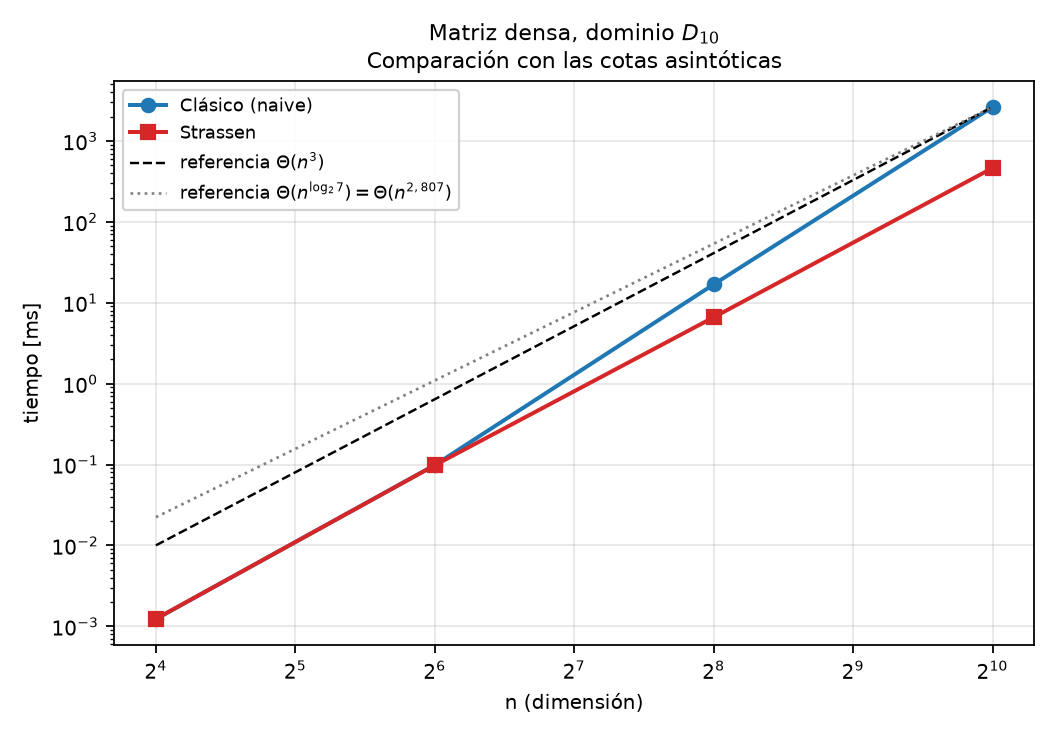
\includegraphics[width=\textwidth]{../code/matrix_multiplication/data/plots/matrix_time_dense.png}
  \end{minipage}\hfill
  \begin{minipage}[b]{0.32\textwidth}
    \centering
    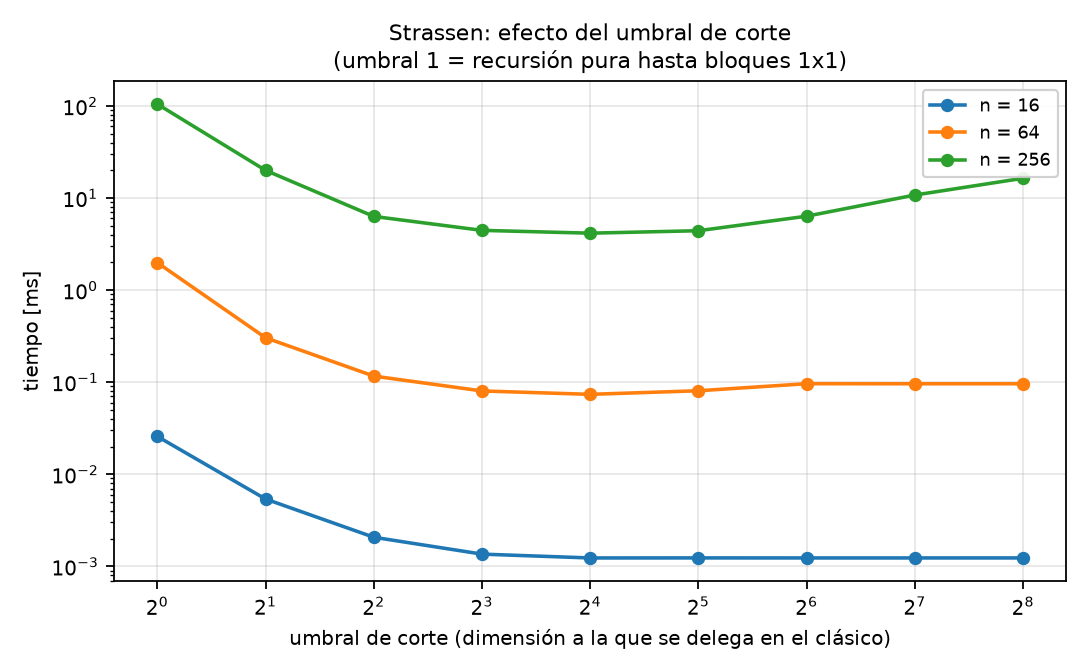
\includegraphics[width=\textwidth]{../code/matrix_multiplication/data/plots/matrix_cutoff_sweep.png}
  \end{minipage}
  \caption{Izquierda: tiempo frente a $n$, matrices densas, con las cotas
  teóricas ancladas al último punto del clásico. Derecha: efecto del umbral de
  corte de Strassen (mediana sobre tipos y dominios).}
  \label{fig:matrix}
\end{figure}

\textbf{Strassen gana, pero sólo cuando $n$ es grande.} En la
\Cref{tab:matrix-time} ambos algoritmos son indistinguibles para $n=2^{4}$ y
$n=2^{6}$ —con el umbral en \MatCutoff{} la recursión no llega a activarse y
Strassen \emph{es} el método clásico— y luego se separan: $\MatSpeedupMid$
veces más rápido en $n=2^{\MatNMidLog}$ y $\MatSpeedupMax$ veces en
$n=2^{\MatNMaxLog}$ ($\MatStrassenMaxMs$ frente a $\MatNaiveMaxMs$~ms). El
punto de cruce está entre $2^{6}$ y $2^{8}$ y la ventaja crece con $n$, como
corresponde a una diferencia de exponente. Se paga en memoria: para
$n=2^{\MatNMaxLog}$ el clásico usa \MatNaiveMemMax{} —exactamente la matriz
resultado, $8n^{2}$ bytes— y Strassen \MatStrassenMemMax{}, $\MatMemRatio$
veces más, por los siete productos y dos acumuladores de cada nivel.

% =============================================================================
% INF-221 Algoritmos y Complejidad -- Tarea 1 -- Semestre 2026-2
% Autor: Kurt Wiederhold   Rol: 202473528-4
%
% ARCHIVO GENERADO AUTOMATICAMENTE por
% code/matrix_multiplication/scripts/plot_generator.py a partir de
% data/measurements/matrix_multiplication_measurements.csv. No editar a mano:
% se regenera con `make plots`.
% =============================================================================
\begin{table}[H]
\centering
\small
\caption{Control (\texttt{make stride-check}): tiempo y costo por operación del clásico, matrices densas $D_{10}$, en $n=2^{k}$ y en dimensiones vecinas de igual memoria; sólo cambia el alineamiento del salto de $8n$ bytes.}
\label{tab:matrix-stride}
\begin{tabular}{lrrrrrrrrr}
\hline\hline
$n$ & 250 & $\mathbf{256}$ & 260 & 500 & $\mathbf{512}$ & 520 & 1000 & $\mathbf{1024}$ & 1040 \\
\hline
tiempo [ms] & 5{,}06 & 16{,}66 & 5{,}53 & 58{,}66 & 363 & 69{,}48 & 497 & 3174 & 533 \\
$t/n^{3}$ [ns] & 0{,}32 & 0{,}99 & 0{,}31 & 0{,}47 & 2{,}70 & 0{,}49 & 0{,}50 & 2{,}96 & 0{,}47 \\
\hline\hline
\end{tabular}
\end{table}


\textbf{Los exponentes medidos superan a los teóricos, y la causa no es la que
parece.} El ajuste $t=c\,n^{p}$ sobre las matrices densas da $p=\MatExpNaive$
para el clásico (teoría: $3$; $R^{2}\ge\MatRsqNaiveMin$) y $p=\MatExpStrassen$
para Strassen entre los \MatExpStrassenPts{} tamaños en que su recursión está
activa (teoría: $\log_2 7=2{,}807$). La explicación inmediata —«la matriz deja
de caber en caché»— queda descartada por el control de la
\Cref{tab:matrix-stride}: matrices de $\MatStrideNeighLo$ y $\MatStrideNeighHi$
ocupan la misma memoria que una de $\MatStrideN$ y tampoco caben en L3, pero
el clásico las multiplica a $\MatStrideNsNeighMin$--$\MatStrideNsNeighMax$~ns
por operación, mientras que en $\MatStrideN$ cuesta $\MatStrideNsPow$~ns:
$\MatStrideFactor$ veces más. Lo que cambia entre esos tamaños es sólo el
\emph{stride}: el bucle interno recorre $B$ por columnas y, cuando $n$ es
potencia de dos, el salto de $8n$ bytes es múltiplo del tamaño de página. El
mecanismo estándar para ese patrón~\cite{drepper2007} —todos los elementos de
una columna caen en el mismo conjunto de la caché (L1d: 64 conjuntos de 64~B)
y, con 8 vías, cada acceso falla aunque la matriz quepa— es consistente con lo
medido, aunque aquí no se contaron fallos de caché. Entre tamaños no potencia
de dos, $t/n^{3}$ varía sólo $\MatStrideNonPowRatio\times$ de $250$ a $1040$
(ese sí sería el efecto de capacidad), frente a $\MatStridePowRatio\times$ de
$256$ a $1024$. Strassen sufre menos,
presumiblemente porque sus operandos temporales son contiguos, pero sus hojas
también leen bloques de $B$ con stride $8n$; de ahí su $p>\log_2 7$. La
consecuencia es importante: al costo por operación de sus vecinos, el clásico
tardaría $\approx\MatStrideEquivMs$~ms en $n=2^{\MatNMaxLog}$ y la ventaja de
Strassen sería de $\MatStrideEquivSpeedup\times$, no de $\MatSpeedupMax\times$:
buena parte de su «triunfo» es el castigo de la caché al clásico en las
potencias de dos.

\textbf{Sin umbral de corte, Strassen no sirve} (curva en U del panel derecho
de la \Cref{fig:matrix}). Para $n=2^{\MatSweepNLog}$ (densa $D_{10}$), la
recursión pura hasta bloques de $1\times1$ tarda $\MatSweepPureMs$~ms:
$\MatSweepPureOverNaive$ veces más que el clásico. El óptimo medido está en el
umbral $\MatSweepBestCut$, con $\MatSweepBestMs$~ms ($\MatSweepNaiveOverBest$
veces más rápido que el clásico); el umbral \MatCutoff{} usado en el resto del
experimento da $\MatSweepDefaultMs$~ms, razonable pero no óptimo: este
parámetro se mide, no se supone. Las 18 sumas de bloques y la asignación de
memoria por nivel son $\Theta(n^{2})$ con constante alta y en bloques pequeños
dominan el ahorro de $8\to7$ multiplicaciones~\cite{husslederman1996}.

\textbf{La estructura de la matriz no importa; el estado de la máquina, sí.}
Como ninguno de los dos algoritmos inspecciona los coeficientes, una matriz
diagonal debe costar lo mismo que una densa, y así ocurre: para
$n=2^{\MatNMaxLog}$ el clásico varía un $\MatTypeDispMain$\% entre los seis
pares tipo/dominio de la corrida principal, y el mismo $\MatTypeDispCtrl$\% se
obtiene al medir cada tipo en un proceso independiente y siempre en primera
posición (\texttt{type\_order\_check.py}: $\MatCtrlDensaMs$, $\MatCtrlDiagonalMs$
y $\MatCtrlDispersaMs$~ms), lo que descarta que el orden de las mediciones
explique la diferencia~\cite{mcgeoch2012}. El control mostró además algo que
no se buscaba: sus tres tiempos son un $\MatCtrlShiftPct$\% más altos que los
mismos casos de la corrida principal. Afecta por igual a los tres tipos y no
altera la conclusión; su causa no se determinó, y por eso este informe sólo
compara mediciones de una misma corrida.
